\chapter{Grammatical Questions}
\label{sec:grammar}

\section{Grammar Topics}
\label{sec:topics}

There is a variety of difficulties German L2 learners encounter while acquiring the language. Some of the typical mistakes and misunderstandings might also be connected to learners language background and be an effect of language transfer [CITE LANGUAGE TRANSFER]. The book ``Mitsprache fördern'' [CITE MITSPRACHE FOERDERN] provides a number of topics that present challenges for non-native speakers of German studying at German schools. The set of topics takes into account different language backgrounds of students.

Not every topic could easily result into an interactive exercise which the user can accomplish while listening to the song. For this reason, such topics as \textit{Verb positioning in main and subordinate clauses} or \textit{Separable and inseparable verbs} were not included in the app. The following topics were considered best suitable for the format of exercises: \textit{Prepositions and their cases}, \textit{Verb conjugation}, \textit{Verb with prefixes} and \textit{Passive voice}.

\subsection{Prepositions and their cases}

Native speakers usually intuitively choose the right case for words in a prepositional phrase. Learners of German, however, have to memorize rules on case usage and practice them with suitable exercises [CITE MITSPRACHE FOERDERN]. Another characteristic of German language that makes the choice of the right case even more difficult is the importance of context for some prepositions [CITE MITSPRACHE FOERDERN]. Such prepositions can be used both with accusative and dative cases e.g. \textit{Der Igel ist \textbf{in den} Garten gegangen} and \textit{\textbf{Im} dunklen Garten faucht und schmatzt es laut}.

Even though the exercises offered in the section \textit{Prepositions and their cases} are limited to local and temporal prepositions, there is no such limitation for the prepositions used in exercises in the app. Not only local (\textit{in} in \textit{Ich spring' in Singapur \textbf{in} das kalte Wasser}) and temporal (\textit{nach} in \textit{\textbf{Nach} all diesen Jahren immer ohne Plan fahren}), but also e.g. modal (\textit{mit} in \textit{Also wieder \textbf{mit} dem Fahrrad auf die Autobahn}) and causal (\textit{wegen} in \textit{Bist mitten in der Nacht \textbf{wegen} mir aufgewacht}) prepositions are taken into account. 

Nevertheless, a prepositional phrase in a song should comply to certain rules. Firstly, a preposition's object should be either a noun or a pronoun e.g. \textit{Blick} in \textit{Verlier' mich in deinem \textbf{Blick}} or \textit{dir} \textit{Ich träum dabei von \textbf{dir}}. 
Secondly, if the preposition's object is a noun, there should be a modifier of the object that illustrates the case that the preposition requires. For instance, such modifier could be an article (\textit{die} in \textit{Atemlos durch \textbf{die} Nacht}), a possessive pronoun (\text{ihrem} in \textit{Hätt' von \textbf{ihrem} letzten Geld [Die Karte heut' gekauft]}) or a preposition itself --- to be precise, a contraction of the preposition with the definite article (\text{zum} in \textit{Schenk' dir 'n Song \textbf{zum} Geburtstag}). Therefore, such prepositional phrases as \textit{mit Schaschliksoße} in \textit{[Sie reden von den alten Werten] \textbf{Mit Schaschliksoße} in den Bärten} were not taken into account. In a similar way, constructions like \textit{Mit Bombenlegern} in \textit{[Ich werde niemals wieder U-Bahn fahren] \textbf{Mit Bombenlegern} aus Islam} have been avoided, even though \textit{-n} in \textit{Bomberlegern} implies that the preposition requires dative case.

Thirdly, the modifier of the object that illustrates the case should have a full form. For this reason, for instance, a prepositional phrase \textit{von unser'n autonomen Fans} in \textit{Weil wir uns nicht distanzier'n von \textbf{unser'n} autonomen Fans} would not be considered proper.

Finally, no constructions with proper nouns are included, as learning gender of proper nouns is considered a secondary priority for German L2 learners. In most cases, gender of noun is needed to use the right form of its modifiers e.g. for choosing \textit{die} in \textit{Atemlos durch \textbf{die|den|das} Nacht}.

\subsection{Verb conjugation}

The section on verb conjugation includes a few exercises on the perfect tense, but it is mainly concentrated on the present and the past tenses [CITE MITSPRACHE FOERDERN]. In the app, among the present (\textit{drehst} in \textit{Und du \textbf{drehst} dich in deiner kleinen Welt}), the past (\textit{ließ} in \textit{Ich \textbf{ließ} die Sonne nie untergehen}) and the perfect tenses (\textit{hast abgenommen} in \textit{Unsere Fotos \textbf{hast} du \textbf{abgenommen}}), also the pluperfect tense (\textit{hattest vorgetrunken} in \textit{[Du warst ein bisschen drauf] Und \textbf{hattest vorgetrunken} [Vodka mit deinen Freunden]}) is taken into account. No preference to any tense is exhibited --- the frequency of forms in a certain tense depends only on the song texts. 

The distinction between irregular and regular verbs\footnote{According to [CITE HAMMER'S GRAMMAR], both strong and weak verbs can be divided into regular and irregular verbs. Here, the term \textit{irregular} includes all strong verbs and irregular weak verbs} deserves special attention in this topic. Although one could argue that more time should be invested into learning irregular verb forms, being exposed to generalizations and learning regular patterns is at least as important. The study [CITE SCHMIDT] illustrates that well. The subject of study, a native Japanese speaker who moved to Hawaii learned English for three years mainly by speaking it and acquired a rather high level of fluency. His grammatical competence was, however, rather limited --- for instance, he was able to use irregular verb forms in past tense, but was unable to make past forms of regular verbs. Therefore, all verb forms have to be present in the app to expose the user to both irregular and regular patterns.

As for prepositional phrases, there is a set of limitations for verb forms. Firstly, forms of \textit{sein}, \textit{haben} and \textit{werden} were not extracted. Forms of the perfect and the pluperfect tenses are an exception for the rule --- in this case, the whole form including both an auxiliary and a main verb would be extracted e.g. \textit{Und heute \textbf{bin} ich \textbf{aufgewacht}}. Modal auxiliary verbs --- \textit{müssen}, \textit{können}, \textit{sollen}, \textit{dürfen}, \textit{wollen}, \textit{mögen} --- were also excluded. 

Secondly, no verb forms that are exclusively used in spoken German were extracted e.g. \textit{hab'} in \textit{Ich \textbf{hab'} den YouTuber-Look, wie im Buche gedruckt}; \textit{zeig} in \textit{Deshalb \textbf{zeig} ich was ich kann an dem verdammten Mikrofon} or \textit{geh'n} in \textit{Komm, wir \textbf{geh'n}}. Forms of the perfect tense with spoken versions of auxiliaries were also avoided, for example \textit{hab' erkannt} in \textit{Ich \textbf{hab'} 'nen Nazi am Geruch erkannt}. Developing the ability of students to use widely accepted written forms in speech is considered more important than extracting all possible constructions from song texts. Moreover, no special knowledge is needed to understand such spoken forms, as they are similar enough to proper forms. Therefore, there is no need for a German L2 learner to memorize them. Apart from logical reasons, there is also a practical reason not to extract verb forms which are used only in spoken German. The parser used to extract verb forms\footnote{On parsers see the section \ref{sec:tools}} always split the word on the apostrophe, which sometimes led to wrongly determined infinitive of the verb. In case of topic \textit{Verb conjugation}, infinitives are necessary for generating distractors. 

Due to homonymy of verbs in imperative mood and verb forms of 1st person singular used in spoken German, in some cases it was not clear if the verb form should be extracted, even when taking into account the surrounding context. For example, \textit{lass} in \textit{Dein Wort hält Wort, \textbf{lass} alle Schatten fort} could be read as \textit{(ich) lass' alle Schatten fort} or as \textit{lass (du) alle Schatten fort}. In such cases, a word was considered a verb in imperative mood and was, therefore, extracted.

Thirdly, contractions of \textit{es} with a verb like \textit{hat's geschrieben} in \textit{Aber wär' auch traurig, mein', er \textbf{hat's} ja auch für dich \textbf{geschrieben}} were also avoided. It was assumed that such contracted forms would move focus from the verb form to contraction.

Fourthly, a verb form was selected even if its prefix was written separably --- for instance, \textit{fängt} in \textit{Du, dich \textbf{fängt} niemand ein}. The decision was based on the fact that verbs that share the same root, regardless of having or not having a prefix, are conjugated in the same way. Thus, a form of 3rd person singular of \textit{fangen} is \textit{fängt}, and of \textit{einfangen} --- \textit{fängt ein}, or \textit{einfängt}.

The last but not the least, if there was several past participles that share the same auxiliary verb e.g. \textit{Du \textbf{hast} mich \textbf{angezogen}, \textbf{ausgezogen}, \textbf{großgezogen}}, only the first participle together with the auxiliary was extracted. In the highlight mode of the app, it is important to perceive a past participle and an auxiliary verb as one verb form, which would not be possible if all the participles are extracted.

\subsection{Verb with prefixes}

The section on systematic vocabulary expansion presents such methods of word derivation as adding prefixes or suffixes and compounding [CITE MITSPRACHE FOERDERN]. Many exercises in the section are solely devoted to verb prefixing and changes in meaning that these prefixes lead to. Due to the difference in meanings, verbs with prefixes proved to be suitable distractors for multiple choice questions.

The following criteria were created for extracting verbs with prefixes from song texts. Firstly, inseparable as well as separable verbs were extracted e.g. inseparable verb \textit{erzählst} in \textit{Von deinem Job \textbf{erzählst} du gar nichts oder wenig} or separable \textit{weitergehen} in \textit{Das ist ein Unding, so kann das nicht \textbf{weitergehen}}.

Secondly, only separable verbs that are written together with their prefixes were selected --- it is claimed that the user would benefit more from perceiving a simple verb\footnote{In [CITE HAMMER'S GRAMMAR], the term \textit{simple verb} means a verb without a prefix} and a prefix as one unit. Separable verbs and their prefixes are written together, for instance, when the verb is an infinitive, as in the example above; when the verb is used in a subordinate clause such as \textit{rumliegt} in \textit{[Und es tut weh, dass man sich nur sieht] Weil bei mir so viel Zeug von dir \textbf{rumliegt}}; or when the verb is used in a form of participle e.g. \textit{abgehört} in \textit{Die NSA hat seit Jahrzehnten jeden \textbf{abgehört}}. 

The third criterion is also connected to separable verbs. Infinitives with \textit{zu} derived from such verbs (e.g. \textit{mitzuteilen} in \textit{Es besteht keine Not einem jedem davon \textbf{mitzuteilen}}) were not extracted, as \textit{zu} would distract attention from the original prefix and might even trick the user into perceiving the original prefix and \textit{zu} as one prefix.

Fourthly, in case of past participles used in combination with an auxiliary (in passive voice, in the perfect tense or in pluperfect tense), only the participle itself is extracted, such as \textit{totgeschlagen} in \textit{Werden sie \textbf{totgeschlagen}, wenn sie kein Kopftuch tragen} or \textit{verändert} in \textit{Denn was hat sich \textbf{verändert} in den letzten fünf Jahren?}. Thus, in highlight mode only parts of verb forms are highlighted. That helps keep focus on prefixes of verbs, and not on their conjugation.

\subsection{Passive voice}

In contrast to spoken language, written language usually presents more challenges for an L2 learner of German. To express thoughts through writing accurately, certain skills are necessary [CITE MITSPRACHE FOERDERN]. One of such skills is usage of passive voice [CITE MITSPRACHE FOERDERN], which can also be trained with interactive exercises in the app.

For the app, passive constructions in the past tense (\textit{wurde geweckt} in \textit{Ich \textbf{wurde} heute morgen von 'nem Panzer \textbf{geweckt}}) and present tense (\textit{wird gemacht} in \textit{Da \textbf{wird} ja schließlich nichts \textit{gemacht}, außer viel Strom verbraucht}) were extracted. Constructions in the perfect tense were avoided due to their complexity e.g. \textit{[Hab Freunde betrogen und 'n paar auch verloren] Frauen verarscht und \textbf{bin verarscht worden}}.

\section{Tools For Extracting Grammatical Constructions} \label{sec:tools}

In order to extract chosen grammatical constructions from song texts, a suitable dependency parser is needed. Four dependency parsers trained on German texts are analyzed in this section: ParZu, spaCy, the Stanford Parser and the Mate tools parser.

\subsection{Dependency parsers}

ParZu \citep{Rico.2009} was trained on Europarl and includes the following components in its pipeline: sentence segmentation, tokenization, part-of-speech (POS) tagging, morphological analysis and the core component --- dependency parser, with a preprocessing step before and a postprocessing step after it. Remarkably, for all the tasks except dependency parsing, ready-made tools were chosen e.g. the punkt\_tokenizer from NTLK was used for tokenization, and clevertagger\footnote{\url{https://github.com/rsennrich/clevertagger}} --- for POS-tagging. The POS-tagger uses the Stuttgart-Tübingen Tag Set (STTS). The dependency analysis is represented in the CoNNL dependency format and includes an index, a lemma, a POS-tag, a language-specific POS-tag, morphological features, a head and a dependency relation for every token. The three other parsers use a similar set of features.

spaCy\footnote{\url{https://spacy.io/}} was trained on TIGER Corpus and WikiNER dataset, and it provides two models for parsing German texts: \textit{de\_core\_news\_sm} (the small model) and \textit{de\_core\_news\_md} (the medium model), with \textit{de\_core\_news\_md} performing with a higher accuracy. Linguistic features supported by spaCy include sentence segmentation, tokenization, POS-tagging, dependency parsing, and named entity recognition. Unlike other parsers, it does not assign morphological features to tokens in languages other than English. Both the POS-tagger and the dependency parser use the TIGER Treebank annotation scheme.

The Stanford Parser \citep{Qi.2018}, which was trained on the Negra corpus, offers a Python package that makes the software easy to install and to use. The neural pipeline of parser in the Python package includes tokenization, multi-word expansion, lemmatization, POS-tagging, morphological features tagging, and dependency parsing. The TIGER variant of STTS is used for POS-tagging, and grammatical relations are defined according to the Universal Dependencies representation\footnote{\url{http://universaldependencies.org/docsv1/}}.

The Mate tools provide a transition-based dependency parser with joint POS-tagging and labeled dependency parsing \citep{Bohnet.2012}. The German models, therefore, include a lemmatizer model and a joint parsing model consisting of the tagger, morphology and parser parts. Before applying the Mate tools to a text, it should be transformed into one-word per line 2009 CoNNL format\footnote{\url{http://ufal.mff.cuni.cz/conll2009-st/task-description.html}} and tokenized. Although the Mate tools provide the script for the first transformation, they do not include a tokenizer. It is suggested to use an OpenNLP library\footnote{\url{https://opennlp.apache.org/}} for that.

To test how well the parsers analyze lyrics, a song text of \textit{Splitter von Granaten} by Adam Angst was used. It was randomly chosen from the lyrics containing all the four types of grammatical constructions.

Before comparing analyses of the four parsers, the best spaCy model needed to be chosen. Texts of songs are quite different from newspaper texts or Wikipedia articles that the models were trained on, so in order to make the best choice, analyses of two models were compared.

Before applying a parser to the text, it was transformed in the way that every line of lyrics was represented as a separate sentence --- either by preserving the punctuation mark in the end of the line or by inserting a full stop. Despite that, the small model split the sentence \textit{Keine Nachbarn Nachts über Grenzen fliehen} into two parts: \textit{Keine Nachbarn} and \textit{Nachts über Grenzen fliehen}. The medium model perceives the sentence as a whole. 

There were a number of cases when analysis of the small and the medium models differ. Analysis of punctuation marks was not taken into account, as it is not relevant for extracting grammatical constructions. Not including punctuation marks and tokens from the sentence \textit{Keine Nachbarn Nachts über Grenzen fliehen}, which was split differently by the two models, thirty-nine cases were detected. The medium model was preferred, as it correctly analyzed twenty-one tokens, compared to thirteen by the small model.

Analyses of the four parsers exhibit some general differences and similarities, not necessarily connected to a certain grammatical construction. For instance, as has already been mentioned above, spaCy is the only parser that does not provide tokens with morphological characteristics. Morphological analysis of the Stanford Parser is easier to read than the analysis of ParZu and the Mate tool, as names of features are specified e.g. \textit{Case=Acc|Gender=Masc|Number=Sing} for \textit{Applaus} in \textit{Und die Welt spendet Applaus}. 

Compared to spaCy, ParZu has more specific dependency relations inside the noun phrase --- many tokens that are analyzed as \textit{nk} (noun kernel) by spaCy have different relations in analysis by ParZu e.g. \textit{det} (determiner), \textit{attr} (attributive) or \textit{pn} (preposition complement). Dependency relations assigned by the Stanford Parser, however, are even more specific than the ones by ParZu. For instance, relation of adjective to noun is \textit{amod} (adjectival modifier), and of cardinal number to noun --- \textit{nummod} (numeric modifier), while both of the relations are marked \textit{attr} in the analysis of ParZu. 

The tokenizer by the OpenNLP library, which is recommended by the Mate tools, does not behave completely usual, compared to tokenizers of other parsers --- for example, it treats two sentences with the question mark after the first sentence as one sentence. Moreover, it splits the line \textit{Asylbewerberheime sind doch sicher, alles klar... 43 Anschläge und dass in einem Jahr} in two sentences, with the first sentence ending with an ellipsis. ParZu, spaCy and the Stanford Parser treat this line as one sentence.

In the next subsections, more specific differences between the analyses of the four parsers are discussed.

\subsection{Prepositions and their cases}

The Stanford parser is the only parser that transforms a contraction of a preposition with the definite article e.g. \textit{am} or \textit{aufs} in two separate words in its analysis. If a combination is non-standard, however, it is treated as an adverb. That makes it impossible to extract constructions like \textit{zum Vergnügen} or \textit{unterm Tellerrand} using the Stanford parser.

In contrast to ParZu, no case is assigned to prepositions in the Stanford Parser and the Mate tools. Moreover, the Mate tools, unlike the three other parsers, assigns some of the tokens wrong morphological characteristics. Therefore, some of the rules cannot include morphological features of tokens, as it would lead to missing some of the constructions.

ParZu seems to be the best tool for extracting prepositional phrases, as its analyses are right, compared to the Mate tools, and it is able to extract constructions like \textit{zum Vergnügen} and \textit{unterm Tellerrand}, in contrast to the Stanford parser. Apart from that, unlike spaCy, ParZu includes morphological information, which helps to describe prepositional phrases that need to be extracted more precisely.

\subsection{Verb conjugation}

First of all, finite verb forms should have right language-specific POS-tags, so that they could be extracted. However, in order to generate distractors for such verb forms, their morphological characteristics and their infinitives are also needed. Therefore, all these three features should be taken into account while choosing a parser. spaCy does not provide morphological information, so it is not suitable for the current topic. Nevertheless, it was compared to other parsers to show how well it deals with other aspects of grammar analysis.

There is no dependency parser that analyzed all the finite verb forms in the right way. With twenty-eight verb forms to extract in total, spaCy assigned wrong language-specific part-of-speech tags to six of them --- for instance, \textit{provoziert} in \textit{Das 'nen Atomkrieg \textbf{provoziert} und denkt es wäre 'ne Kissenschlacht} is tagged \textit{VVPP} (perfect participle, full) instead of \textit{VVFIN} (finite verb, full). Other examples include cases when a verb was tagged \textit{VVFIN} instead of \textit{VVPP} and \textit{VVINF} (infinitive, full) instead of \textit{VVFIN}.  Two of the verbs have wrong infinitives --- for example, \textit{taten} in \textit{Und wir \textbf{taten} überrascht und waren 'ne Woche lang empört} was assigned infinitive \textit{taten} instead of \textit{tun}. In total, eight out of twenty-eight verbs were analyzed wrong by spaCy.

In case of ParZu, five verbs were assigned wrong language-specific POS-tags. As in analyses by spaCy, some of them were tagged \textit{VVINF} instead of \textit{VVFIN} and some --- \textit{VVPP} instead of \textit{VVFIN}. ParZu does not provide any wrong morphological analysis, but for a few verb forms, some morphological features were not determined e.g. \textit{geht} in \textit{Doch worum es gerade \textbf{geht} wissen wir selbst nicht so genau} is not assigned neither number nor person. Cases when only mode was not determined were not considered a mistake --- for instance, \textit{wissen} from the previous example was not assigned any mode. From analyses of a greater number of songs with the parser, it could be concluded that for every such case the indicative mode could be assumed. Thus, including the verb \textit{abgehört} in \textit{Die NSA hat seit Jahrzehnten jeden \textbf{abgehört}} that was assigned a wrong infinitive \textit{abgehören}, ten out of twenty-eight verbs were analyzed wrong by ParZu.

In the analysis by the Stanford parser, the following mistakes could be found. Two of the verbs were assigned wrong language-specific characteristics and got tagged \textit{VVINF} instead of \textit{VVFIN}. This mistake occurs in analyses of all parsers, including the Mate tools. For example, \textit{springen} in \textit{[Solang hier keine Sirenen erklingen] Keine Soldaten durch unsere Fenster \textbf{springen}} was wrongly assigned tag \textit{VVINF} by the Stanford parser, ParZu and spaCy. One other verb, \textit{taten} in \textit{Und wir \textbf{taten} überrascht und waren 'ne Woche lang empört} which also posed challenges to spaCy, was assigned wrong morphological features and a wrong infinitive. All in all, analyses of only three out of twenty-eight verb forms contained mistakes in case of the Stanford parser.

Analysis by the Mate tools contains a number of various mistakes. One of the verbs was assigned wrong morphological features, another one --- a wrong infinitive, while the third one, \textit{schießen} in \textit{Polizisten ticken aus und \textbf{schießen} wahllos in die Menge} had a combination of both these mistakes. Two other verbs were not assigned any morphological characteristics at all. Finally, language-specific POS-tag for one of the verbs was selected wrong. Therefore, six out of twenty-eight verbs were assigned wrong analysis by the Mate tools.

As has been mentioned above, not only POS tags, but also morphological features of verbs are important for extracting finite verb forms. Therefore, taking into account results of parsers that provide morphological information about word forms, the best parser for extracting finite verb forms is the Stanford Parser.

\subsection{Verbs with prefixes}

For getting a list of verbs with prefixes from a song text, candidates for such verbs should be identified first. That is exactly why the analysis from a dependency parser is needed --- to get all possible verb forms that then will be tested for having a prefix. 

It is worth mentioning that extraction of verbs with prefixes is rather similar to extraction of finite verb forms. One of the differences is including forms in passive voice for verbs with prefixes and excluding them for verb conjugation, as verb forms in passive voice is a grammar topic on its own. Another difference would be infinitives, which can serve as candidates for verbs with prefixes, but do not constitute a finite verb form. Moreover, in contrast to verb conjugation, infinitives and morphological characteristics are not needed for generating distractors for the current topic. Therefore, it was decided to analyse results of parsers for the two topics separately.

As neither morphological features nor infinitives are taken into account, the main criterion to choose the most suitable parser is its ability to assign right language-specific POS-tags. 

In analyses of spaCy, ParZu and the Mate tools, some verb forms were assigned a wrong language-specific part-of-speech --- for example, \textit{erklingen} in \textit{Solang hier keine Sirenen erklingen} is assigned tag \textit{VVINF} instead of \textit{VVFIN} by ParZu or \textit{abgehört} in \textit{Die NSA hat seit Jahrzehnten jeden abgehört} is tagged \textit{VVFIN} instead of \textit{VVPP} by spaCy. In the first example, it is rather clear that the wrong tag was assigned due to ambiguity of the verb form. In the second case, however, the verb forms are not homonymous --- there is no finite verb form \textit{abgehört}. A mistake of the second type is only found in the analysis of spaCy. ParZu and the Mate tools analyze verb forms in a wrong way only if forms have homonyms. There are three mistakes in assigning language-specific POS-tags in the analysis of spaCy, while both ParZu and the Mate tools each produce two such mistakes.

In contrast to parsers discussed above, the Stanford Parser assigns all verb forms right language-specific POS-tags. For this reason, it is considered the best parser for extracting verbs with prefixes.

\subsection{Passive voice}

ParZu, spaCy and the Mate tools do not distinguish perfect tense and passive voice --- namely, the dependency relation between an auxiliary and the main verb is always \textit{aux} (auxiliary verb; in case of ParZu) or \textit{oc} (clausal object; in case of spaCy and the Mate tools). Thus, constructions like \textit{hat verändert} in \textit{Denn was \textbf{hat} sich \textbf{verändert} in den letzten fünf Jahren} and \textit{wird gemacht} in \textit{Da \textbf{wird} ja schließlich nichts \textbf{gemacht}, außer viel Strom verbraucht} would be parsed alike.

The Stanford parser, however, has a special relation for verb forms in passive voice --- \textit{aux:pass}, while for perfect tense the relation would be called simply \textit{aux}.  Therefore, the Stanford Parser is best suitable for extracting constructions for this topic, as well.

To make the conclusion, ParZu will be used for extracting prepositional phrases, and the Stanford Parser --- for extracting constructions for the rest of the topics. However, on the stage of writing rules it would become clear that for some topics, results of analysis of one song should not be generalized for the whole corpus of song texts. For these topics, a parser would be chosen again, this time based on a greater selection of songs.

\section{Manual Tagging and Splitting}

To be able to write rules for extracting grammatical constructions discussed in section \ref{sec:topics} and check them afterwards, all the four construction types --- prepositions and their cases, verb conjugation, verbs with prefixes and passive voice --- were manually tagged in all the song texts. During that process, the limitations described in section \ref{sec:topics} for every topic were met.

After that, songs containing constructions for each type were grouped together. The distribution of constructions of different types can be seen in table \ref{table:songs-to-types}.

\begin{table}[h!]
\centering
    \begin{tabular}{c|c|c|c}
        Prep. and their cases  & Verb conj. & Verbs with pref. & Pass. voice \\
        \hline
        130 & 131 & 121 & 35 \\
        \hline
    \end{tabular}
    \caption{Number of songs with constructions of each type}
    \label{table:songs-to-types}
\end{table}

One could see that verbs and prepositional phrases could be found in all or almost all constructions, while verbs with prefixes occur in 92\% of songs. Verb constructions in passive voice are, however, relatively rare and could be seen in only 27\% of texts.

For each construction type, songs were split into two sets --- one set was used for writing rules for extracting certain type of construction, and the other --- for evaluating rules. Here, these sets would be called with terms often used in machine learning --- \textit{training set} and \textit{test set}. The ratio 20:80 was chosen for the split, following Pareto principle\footnote{\url{https://en.wikipedia.org/wiki/Pareto_principle}}.

It was decided to sample every set with respect to genre of songs, in order to account for possible differences in structure of constructions or in their rate of occurrence among various genres. As stated in section \ref{sec:selection}, participants assigned genres to artists and bands based on their own definition of genres. In two cases, it led to a conflict of genres e.g. some students labeled Rammstein as \textit{Rock}, and other --- as \textit{Metal}. In such cases, the genre was assigned based on the number of people that had chosen every genre. Rammstein was assigned genre \textit{Rock}, as it was the option preferred by most students.

\begin{table}[h!]
    \centering
    \begin{tabular}{l|c|c|c}
        & Total N of songs & Training set & Test set \\
        \hline
        Dance/Electronic/House & 3 & 1 & 2 \\
        Hip-Hop/Rap/Trap & 42 & 8 & 34 \\
        Metal & 3 & 1 & 2 \\
        Pop & 30 & 6 & 24 \\
        Rock & 38 & 8 & 30 \\
        Singer/Songwriter & 14 & 3 & 11 \\
        \hline
        Total & 130 & 27 & 103 \\
        \hline
    \end{tabular}
    \caption{Distribution of songs by genre in training and test sets for construction type \textit{Prepositions and their cases}}
    \label{table:genre-distribution}
\end{table}

Sampling training and test sets by genre for construction type \textit{Prepositions and their cases }can be illustrated by table \ref{table:genre-distribution}. In the same way, training and test sets for other construction types were balanced on music genres.

\section{Rules}

\subsection{Prepositional phrases}

As has been explained in \ref{sec:tools}, ParZu was chosen as the best suitable parser for extracting prepositional phrases from song texts. Before applying the parser on texts, they were prepared in the same way as the song text \textit{Splitter von Granaten} by Adam Angst that was used for choosing a parser for extracting constructions of each type. Namely, to every lyrics line that did not have a punctuation mark at the end was attached a full stop. Then all lines were written as a prose text, with lyrics lines being separated by a space. 

One could argue that representing each line of song lyrics as a separate sentence may lead to errors in parsing. However, only 7\% of lines in all song texts contain a punctuation mark signaling the end of the sentence at the end of the line. For many songs e.g. \textit{Lieder} by Adel Tawil, a comma is the only punctuation mark found in the text. Representing the whole song text as one sentence would, undoubtedly, lead to many more errors than the suggested representation of the song text. For this reason, all lines of song texts were transformed into separate sentences. 

For representing words analyzed by ParZu, class \textit{Word} was written. The class includes all the attributes needed to describe the information the parser provides about word forms: \textit{id} for index of word in sentence, \textit{form} for word form itself, \textit{lemma} for lemma of word form, \textit{upos} for a POS-tag, \textit{xpos} for a language-specific POS-tag, \textit{head} for id of word form's head and \textit{rel} for type of dependency relation of word to its head. Moreover, class \textit{Word} has an attribute \textit{feats} --- a dictionary that contains word form's morphological features. Depending on the part of speech, this dictionary can contain different keys. For instance, for an article the dictionary would only contain its case, and for a finite verb --- its person, number, tense and mode. Class \textit{Word} is also used for representing words constituting rules.

Every rule is usually represented as an array of strings e.g. as in figure \ref{fig:pp-rule}. Strings in a rule get subsequently transformed into instances of Word class --- for this reason, all attributes in strings are separated with a tab, as in words analyzed by ParZu. A string must include a language-specific POS-tag and may include restrictions on morphological features, a head of the word form and the dependency relation of the word form to its head.

\begin{figure}[H]
    \centering
    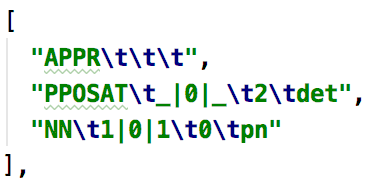
\includegraphics[scale = 1]{images/pp-rule.png}
    \caption{Example of rule for extracting prepositional phrases}
    \label{fig:pp-rule}
\end{figure}

Language-specific POS-tags and types of dependency relations are the same as used in analysis of song texts by ParZu e.g. \textit{PPOSAT} (attributive possessive pronoun) and \textit{det} (determiner). Morphological features, however, instead of looking more specific --- for instance, \textit{Neut|Acc|Pl} (neuter gender, accusative case, plural number), show the agreement between words constituting the construction. For example, as shown in figure \ref{fig:pp-rule}, each \textit{PPOSAT} and \textit{NN} (noun) have three morphological features separated with a vertical bar --- in this case, gender, case and number. Both the pronoun and the noun should, therefore, have the same case as the first element of array (it has index 0), tagged as \textit{APPR} --- the preposition. There are no limitations set on gender and number of the pronoun. However, the noun's gender and number should certainly agree with gender and number of the second element of array (it has index 1), namely, the pronoun. Heads of rule words are also specified relative to the structure of the array. Thus, the possessive pronoun has the third element of array (it has index 2) as its head --- the noun, and the head of the noun is the first element of the array, the preposition.

Apart from containing strings with word's characteristics, as described above, rules can contain a special character \textit{+}, stating that the word described by a previous string could be repeated an unlimited amount of times. Figure \ref{fig:pp-rule-plus} gives an example of such rule, describing a prepositional phrase that includes a preposition, a possessive pronoun, one or more adjectives and a noun.

\begin{figure}[H]
    \centering
    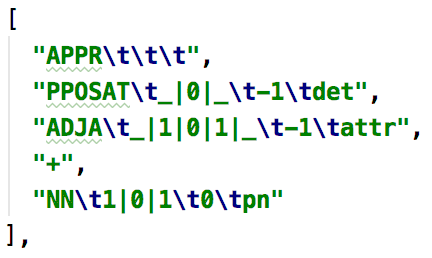
\includegraphics[scale = 1]{images/pp-rule-plus.png}
    \caption{Example of rule with a special character \textit{+}}
    \label{fig:pp-rule-plus}
\end{figure}

To exclude erroneous constructions, it could be useful to set restrictions on lemmas that in some cases lead to extracting a wrong construction. For instance, \textit{bis} in \textit{Willst du \textbf{bis} der Tod euch scheidet [Treu ihr sein für alle Tage?]} is analyzed as a preposition, which leads to extracting \textit{bis der Tod} as a prepositional phrase. A blacklist is introduced as means of excluding constructions with some lemmas from the result. The blacklist is a dictionary, where language-specific parts of speech correspond lists of excluded lemmas.

There is also a way to specify word forms or parts of speech that should not precede or follow certain constructions. For example, extracting \textit{Zum Homo} from the line \textit{\textbf{Zum Homo} Sapiens gehört nicht nur aufrecht geh'n} would be wrong, as the whole prepositional phrase also includes the word \textit{Sapiens}. Theref
Another dictionary, representing a blacklist for words surrounding constructions, helps to avoid such cases.

In total, there are 391 prepositional phrases in the training set, 251 of them are unique. Constructions were considered the same if the word forms constituting them were the same, independent of their surrounding words and the structure of the sentence, as, for instance, the prepositional phrase \textit{um dich} in \textit{\textbf{Um dich} rum lachende Gesichter} and in \textit{[Mit jedem Bissen wird man hungriger, unsicher] Wer man is', weil \textbf{um dich} herum sind alle Wunderkinder}. 

All morphological features of word forms from 86.5\% of these unique constructions are defined, 13.5\%, or 34 unique constructions, however, lack some characteristics. For example, no gender and number is assigned for the possessive pronoun and noun in \textit{auf deine Fragen} (\textit{Kein Bock \textbf{auf deine Fragen}}. The single construction for which a morphological characteristic was defined wrong is also included in these 13.5\% --- \textit{Bett} is assigned nominative case in the prepositional phrase \textit{im Bett} (\textit{Danach, bei dir, du nackt \textbf{im Bett} und ich barfuß am Klavier}). Therefore, two sets of rules were defined: a set of strict rules that are not able to extract these 13.5\% of constructions from the training set and a set of non-strict rules that account for the constructions that lack morphological features. As could be expected, strict rules lead to 34 unique false positives, which result in 45 false positives in total. Non-strict rules yield not only some false positives, but also a few true negatives.

Maintaining high precision is considered more important than achieving a high recall, because providing the user with less correct constructions is definitely more effective for acquiring a certain grammatical topic than getting more correct constructions on the cost of selecting constructions completely not suitable for the chosen grammatical topic. The second case might frustrate the user, and even incline him/her to memorize non-existing rules. Thus, avoiding true negatives should have a higher priority than avoiding false positives, and, if needed, should be done even on the cost of getting more false positives.

For this reason, non-strict rules that led to true negatives were modified. Some of them were made stricter e.g. rule for extracting a prepositional phrase consisting of a preposition, an article and a noun. This rule accidentally extracted construction \textit{für ein Hurensohn} in \textit{Was bist du \textbf{für ein Hurensohn}, sogar die Wurst hat zwei!} and, therefore, was modified by making all word forms in the prepositional phrase to share the same case. Some of non-strict rules were deleted, too --- for instance, the rule used to extract \textit{von der Geschicht'} from \textit{Und die Moral \textbf{von der Geschicht'}: ``Es heißt Geschichte!''} also extracted \textit{nach dem Ende '} from \textit{Ich bin raus, kann schon \textbf{nach dem Ende '}nen Anfang sehen}, while the right prepositional phrase does not include the apostrophe. 

As non-strict set of rules leads to extracting more constructions from song texts, even after some rules were modified, it also shows better results on the training set than the strict set. All in all, 18 unique false positives, which is 20 false positives in total, could not be extracted by the non-strict rules.

A black list is a part of both strict and non-strict sets of rules. One of the members is \textit{bis} which cannot be a preposition, as it leads to extracting \textit{bis der Tod} from \textit{Willst du \textbf{bis} der Tod euch scheidet [Treu ihr sein für alle Tage?]}, as has been already mentioned above. The other member is \textit{paar}, which, unlike other attributive indefinite pronouns with a determiner\footnote{Translation of ``attribuierendes Indefinitpronomen mit Determiner'', term used in the guidlines for tagging texts with the tagset of STTS [CITE GUIDELINES]. This tagset is used by a POS-tagger in ParZu.}, is unable to illustrate the case required by a preposition e.g. \textit{mit paar Homies} in \textit{Ich hock in meinem Viertel \textbf{mit paar Homies} auf 'ner Bank}.

Some constructions were wrongly written in song texts, which hindered the parser to extract them --- for instance, \textit{aufs Licht} in \textit{[Ey, ich sitz' rum völlig dicht, denke an nichts] Und wart' ungeduldig \textbf{aufs Licht</prep>}} was written as \textit{auf's Licht} or \textit{am Gaffen} in \textit{Viel zu viele Menschen um uns rum sind \textbf{am Gaffen}} was written using a small letter, namely \textit{am gaffen}. Such mistakes were corrected in texts, and corrected texts were analyzed by the parser again.

- generalized rules
- test set
- final results

\subsection{Verbs with prefixes}

\subsection{Finite verb forms}

\subsection{Passive voice}